\LARGE{ \textbf {Лекция №8} 2.4.2018}\\
\Large{ \textbf {Двойственные задачи линейного программирования}}

Двойственная задача линейного программирования - это формальная модель обратной по своей структуре
по отношению к исходной прямой постановке задачи.

Для любой линейной задачи можно построить двойственную.
Принято выделять симметричную и несимметричную.

\Large{Прямая задача.}\\
$z = \sum \limits_{j-1}^n c_j x_j $ to MIN.\\
$x_j => 0 \quad j=1...n$\\
$ \sum \limits_{j-1}^n a_{ij} x_j => b_j  \quad j=1...m $\\



\Large{Двойственная задача.}\\
$z = \sum \limits_{i=1}^m b_i y_i $ to MAX.\\
$ \sum \limits_{i=1}^m a_{ij} y_i =< c_j $\\
$y_j => 0 $\\

\Large{Несимметричные пары.}\\
\Large{Прямая задача.}\\
$z = \sum \limits_{j-1}^n c_j x_j $ to MIN.\\
$x_j => 0$\\
$ \sum \limits_{j-1}^n a_{ij} x_j = b_i $\\


\Large{Двойственная задача.}\\
$z = \sum \limits_{i=1}^m b_i y_i \quad $ to MAX.\\
$ \sum \limits_{i=1}^m a_{ij} y_i =< c_i $\\
$y_j >=< 0 $\\

Для приведения несимметричного случая к симметричному.\\
Надо каждое условие равенство заменить 2 неравенствами больше или меньше или равно.\\

Теория двойствености должна обеспечивать возможность решения линейных задач, которые неудобно решать прямым алгоритмом симплекс-метода
из-за сложности выбора опорного базиса. Такое имеет место при ограничениях типа больше или равно.
Потому что в этом случае для перехода в каноническую форму в левую часть этих условий нужно вводить избыточные переменные,
значения которых будут отрицательны в опорном базисе исходных перменных.

Постановка задачи.\\
$-z + \sum \limits_{j-1}^n c_j x_j = 0$\\
$x_j => 0 \quad j=1...n$\\
$ - x_n+i =  b_i  - \sum \limits_{j=1}^n a_{ij} x_j =>  $\\

Двойственная задача.\\


$z = \sum \limits_{i=1}^m b_i y_i $ to MAX.\\
$ \sum \limits_{i=1}^m a_{ij} y_i =< c_j $\\

$ z -\sum \limits_{i=1}^m b_i y_i = 0  $
$y_m+j = c_j - \sum \limits_{i=1}^m a_{ij} y_i => 0 $
$y_j => 0 $\\

Это все при условии, что $c_j => 0$ в исходной задаче.

От прямой задачи перейти к решению двойственной задачи с остаточными дополнительными перменными, которые образуют опорный базис,
то тогда это базис будет допустимым иможно решить двойственную задачу прямым симплекс-методом,
то есть найти оптимальное значение двойственных переменных.\\

После этого нужно восстановить по найденному двойственному оптимальному решению оптимальное решение прямой задачи.
Для этого используется соответсвие между прямыми и двойственными переменными в канонических формах прямой и двойственной задачи.

Прямые свободные соответсвуют базисным двойственным. Но только те, индексы которых совпадают.\\

% Предположим, исходный базис двойственной задачи является оптимальным, тогда получается, что двойственные переменные  ----- , они нам извеснтны, свободные двойственные равны 0.

Использовать соответсвие по индексам прямых и двойственных переменных нужно следующим образом:
допустим, получена оптимальная симплекс таблица двойственной задачи,
тогда коэфиценты её строки целевой функции перед двоственными перменными будут равны значениям прямых перменных,
которые соотвсвуют им по индексам таблицы соответсвия прямых и двойственных перменных.

Для примера, пусть двойственная переменная $y_2$ , которая в исходной задаче была свободна соотвествует прямой переменной $x_4$ ,
которая в исходном прямом базисе была базисной.
В оптимальном базисе двойственной задачи эта перменная, предположим стала базисной.
В этом случае в симплекс таблице коэфицент перед ней равен 0,
а это означает, что соответсвующая прямая переменная будет в своем прямом базисе свободной со значением 0.

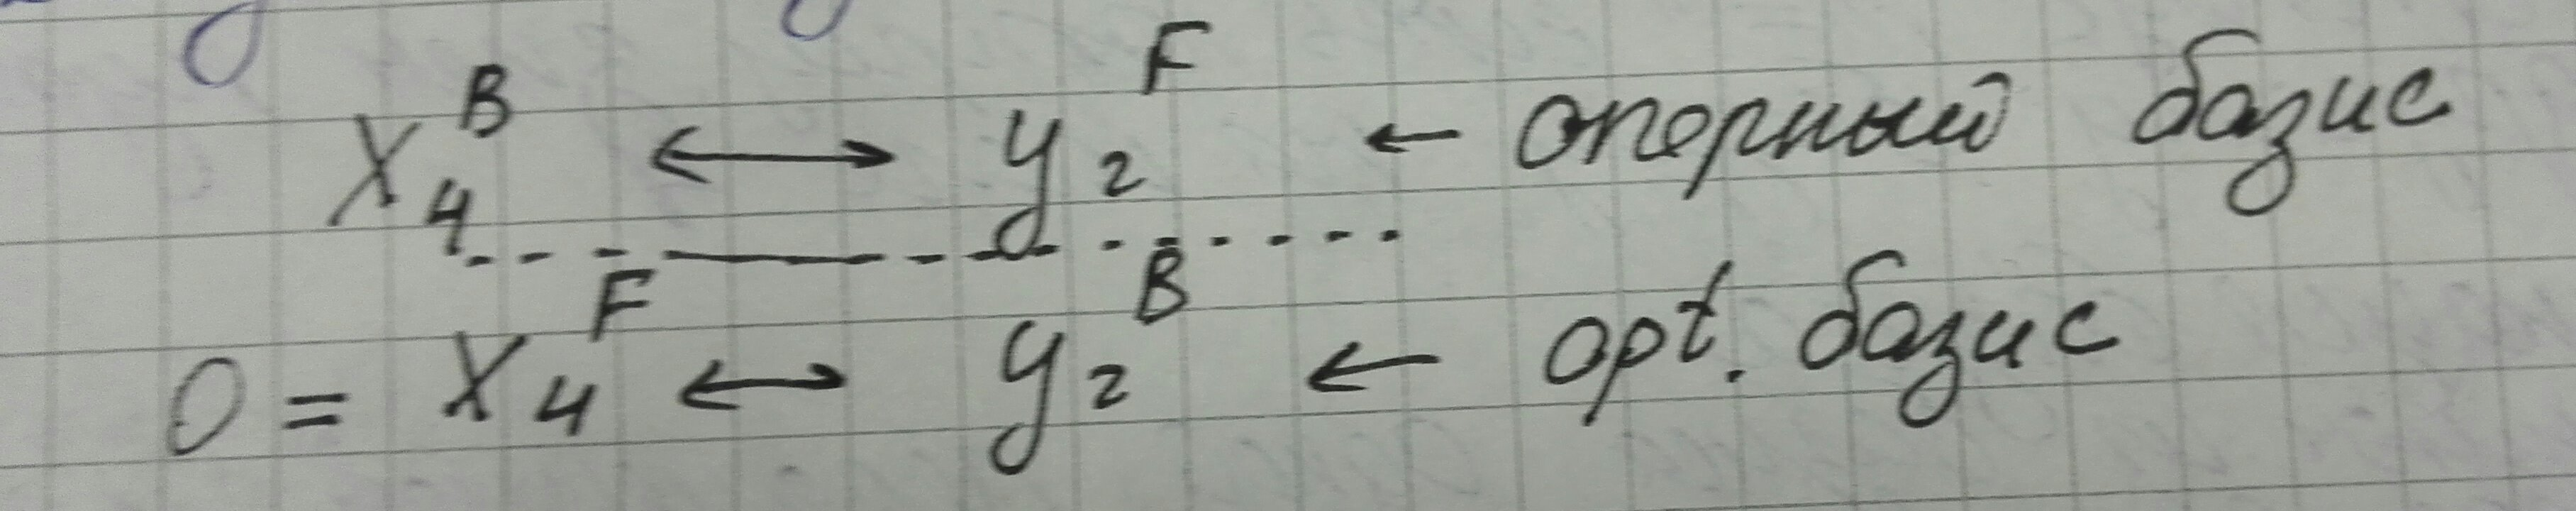
\includegraphics[width=\linewidth]{2}



\Large {Двойственный алгоритм симплекс-меода.}\\

1) Нужно начать с опорного двойственно-допустимого базиса, который является допустимым решением двойственной задачи.
При этом постановка прямой задачи записывается  в канонической форме диагональной относительно критереальных и базисных переменных.
$ x_0 + \sum \limits_j A_0j x_j^F = A_00 $\\
$x_n+i ^B +  \sum \limits_j A_ij x_i^F = A_i0 $\\

Обычно за базисные перменные принимают остаточные и избыточные, а исходные переменные являются свободными,
при этом каждое уравнение с избыточыми перменными нужно умножить на -1 , чтобы коэфицент перед ней вместо -1 стал +1.
Разумеется при этом изменяться знаки других коэфицентов исвободого члена, который будет отрицатеьным, это означает, что такое решение не является прямо допустимым, но ему будет соответсвовать допустимое решение двойственной задачи.
Таким образом это решение будет двойственно допустимым.
При двойственно допустимом базисе  все коэфиценты z должны быть неотрицательными. -----

2) Нужно  предстваить диагональную форму относительно текущего базиса в форме симплекс таблицы,
который имеет такой же формат, как в прямом алгоритме симплекс-метода.


3) Нужно оценить оптимальность текущего базиса по правым частям ограничений,
то есть по коэфицентам в столбце равно симплекс таблицы. Базис будет оптимальным,
когда все правые части станут неотрицательны, а неотрицательность коэфицентов в строке z гарантировано сохраняется на всех итерациях.


Прямо-двойственно допустимый базис.\\
Дв + Пр = Оптимальный базис.\\
Если такой базис достигнут, то итерации нужно завершить и перейти на шаг 6.
Если же прямая допустимость нарушена, то есть в столбце = есть отрицательные значения, нужно изменить базис на шаге 4.
$ A_0j => 0 $\\
$ A_i0 => 0 $\\

4) Модификация базиса производится путем исключения из базиса одной перменной, которая делается свободной,
а вместо нее в базис вводится новая, бывшая свободная переменная.
